
%----------------------------------------------------------------------------------------
%	PACKAGES AND THEMES
%----------------------------------------------------------------------------------------

\documentclass{beamer}

\mode<presentation> {
\usetheme{Madrid}
}

\usepackage[english]{babel}
\usepackage[utf8]{inputenc}
\usepackage{lmodern}
\usepackage{amsmath,amsfonts}
\usepackage{csquotes}
\usepackage{textcomp}
\usepackage{graphicx} % Allows including images
\usepackage{booktabs} % Allows the use of \toprule, \midrule and \bottomrule in tables
\usepackage{ccicons}

\usepackage[citestyle=authoryear-comp,bibstyle=authoryear,maxbibnames=5,minbibnames=1,maxnames=4, minnames=1,datezeros=false,date=long,isbn=false,natbib=true,url=false,backend=bibtex]{biblatex}
\addglobalbib{Computing_References.bib}	
%%% define blue highlighting
\newcommand{\highlight}[1]{{\color{blue}{#1}}}

\mode<trans>
{\renewcommand{\highlight}[1]{{\textbf{#1}}}}


\mode<handout>
{
\renewcommand{\highlight}[1]{{\textbf{#1}}}
%\pgfpagesuselayout{2 on 1}[a4paper,border shrink = 5mm]
%\setbeamercolor{background canvas}{bg=black!5}
}

\setbeamertemplate{footline}{
\begin{beamercolorbox}{section in head/foot}
\insertsectionnavigationhorizontal{.95\textwidth}{\hskip0pt
 Programming \hfill}{\hfill \insertframenumber /\inserttotalframenumber}\href{http://creativecommons.org/licenses/by-sa/4.0/legalcode}{\ccbysa}
\end{beamercolorbox}
}

\usepackage{hyperref}
\hypersetup{bookmarksnumbered=true,naturalnames=true,pdfhighlight=/N,citebordercolor={1 1
1},linkbordercolor={1 1 1},colorlinks=true,anchorcolor=black,linkcolor=blue,citecolor=black,
pdfpagemode=UseThumbs, pdfpagelayout=TwoColumnLeft,breaklinks=true, pdftitle=Scientific Computing,
pdfsubject=Macroeconomics,pdfstartpage=1,pdfpagemode=UseOutlines} %pdfpagemode=fullpage

%----------------------------------------------------------------------------------------
%	TITLE PAGE
%----------------------------------------------------------------------------------------

\title[Intro to Scientific Computing]{Introduction to Scientific Computing} % The short title appears at the bottom of every slide, the full title is only on the title page
\author{Vahe Krrikyan/Johannes Pfeifer} % Your name
\institute[CDSE] % Your institution as it will appear on the bottom of every slide, may be shorthand to save space
{
University of Mannheim \\ % Your institution for the title page
\medskip
\textit{pfeifer@uni-mannheim.de} % Your email address
}
\date{\today} % Date, can be changed to a custom date

\begin{document}

\begin{frame}
\titlepage % Print the title page as the first slide
\end{frame}

\begin{frame}
\begin{figure}
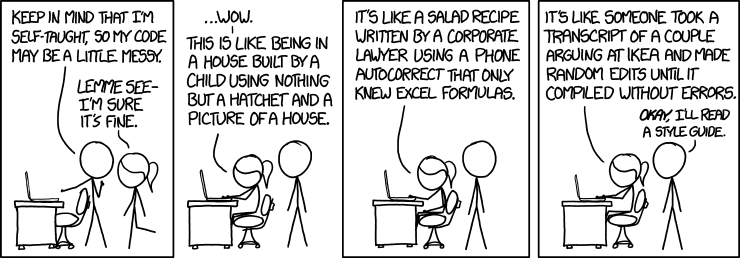
\includegraphics[scale=0.5]{code_quality}
\caption{\url{https://xkcd.com/1513/}}
\end{figure}
\end{frame}

\begin{frame}
\frametitle{Outline} % Table of contents slide, comment this block out to remove it
\tableofcontents % Throughout your presentation, if you choose to use \section{} and \subsection{} commands, these will automatically be printed on this slide as an overview of your presentation
\end{frame}

%----------------------------------------------------------------------------------------
%	PRESENTATION SLIDES
%----------------------------------------------------------------------------------------
\section{Introduction}
%----------------------------------------------------------------------------------------

\begin{frame}
\frametitle{Introduction}
\begin{itemize}
\item This presentation is based on \fullcite{Wilsonetal2014}

\end{itemize}
\end{frame}
%---------------------------------------------------------------------------------------
\begin{frame}
\frametitle{Introduction}
\begin{itemize}
\item Nowadays scientific work almost impossible without scientific computing software
\item Software as important as hardware in modern science and economics in particular
\item Coding is an integral part of economic research, unless purely theoretical (even then software helps checking algebra)
\item Development of Information Technologies, a driver for more sophisticated research techniques
\end{itemize}
\end{frame}
%------------------------------------------------------------------------------------------

\begin{frame}
\frametitle{Introduction}
\begin{itemize}
\item Scientist spend 30\% or more of their time on developing their own software \parencite{Hannayetal2009,Prabhuetal2011}
\item Thus research quality and results highly dependent on developed software
\item E.g. Managing and analyzing large amounts of data, running sophisticated regressions or quantitative experiments
\item Even running simple OLS regressions requires coding
\item Examples of programming languages used in economics: Matlab, Stata, Eviews, R, Fortran, Python, Julia, etc.
\end{itemize}
\end{frame}
%-------------------------------------------------------------------------------------
\section{Motivation}
%-------------------------------------------------------------------------------------

\begin{frame}
\frametitle{Motivation}
\begin{itemize}
\item As already mentioned, significant time of research spent on developing software
\item Thus knowing how to do it right is as important as learning programming.
\begin{itemize}
\item Helps to get more reliable results
\item Decreases the amount of time needed to develop software and boosts the optimality of work
\item Allows for replicability (which increases the validity of the results)
\end{itemize}
\item Mistakes in codes not only dangerous for the quality of the project, but also for those citing it (Domino Effect)
\end{itemize}
\end{frame}
%-------------------------------------------------------------------------------------

\begin{frame}
\frametitle{Motivation}
\begin{itemize}
\item An example for the consequences of mistakes in coding: \fullcite{ReinhartRogoff2010PP}
\item \citet{Herndonetal2014}: ``We replicate Reinhart and Rogoff (2010) and find that \highlight{coding errors, selective exclusion of available data, and unconventional weighting of summary statistics lead to serious errors} that inaccurately represent the relationship between public debt and GDP growth  among 20 advanced economies in the post-war period''.
\item We wouldn't like to be in a situation like this, would we?
\end{itemize}
\end{frame}
%-------------------------------------------------------------------------------------
\section{Best Practices}
%-------------------------------------------------------------------------------------
\begin{frame}
\frametitle{Summary of Best Practices}
A list of suggestions relevant for scientific work in the field of economics
\begin{enumerate}
\item Write a program for people, not computers
\item Let the computer do the work
\item Make incremental changes
\item Don't repeat yourself
\item Plan for mistakes
\item Optimize software only after it works correctly
\item Document design and purpose, not mechanics
\item Collaborate
\end{enumerate}
\end{frame}
%-------------------------------------------------------------------------------------
\begin{frame}
\frametitle{1.Write a Program for People}
\begin{figure}
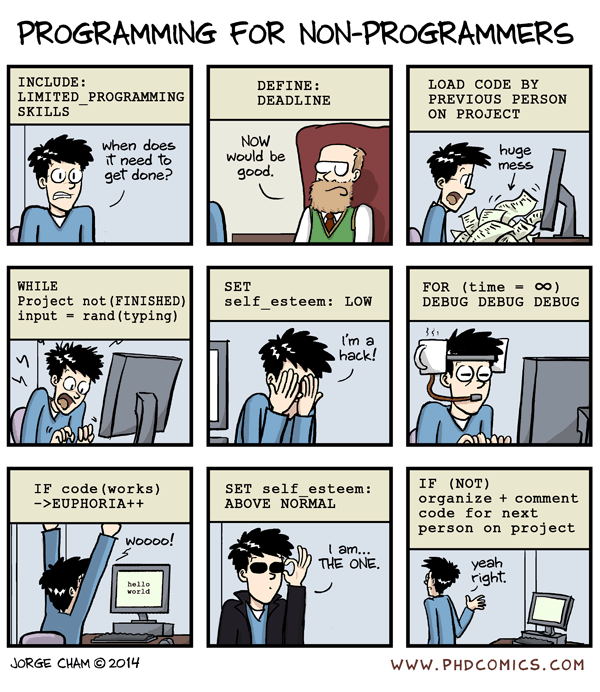
\includegraphics[scale=0.3]{phd031714s}
\caption{\url{http://phdcomics.com/comics/archive.php?comicid=1690}}
\end{figure}
\end{frame}

\begin{frame}
\frametitle{1.Write a Program for People}
\begin{itemize}
\item Software produced by researchers is intended not only to produce correct output, but also be understandable for others and for the researcher himself when he gets back to the code months later
\item Others need to understand the codes so that they can replicate the project.
\item Break the program into separate functions that conduct a separate task - easier for others to understand the program as they concentrate on a limited amount of information at a time.
\item Be consistent with naming the variables: so they are distinctive and informative. \highlight{Don't name variables randomly}.
\item Make code style and formatting consistent: e.g. k\_t\_ss and cSS\_t (c\_t\_ss) inconsistent, harder to read and understand.
\end{itemize}
\end{frame}
%-------------------------------------------------------------------------------------
\begin{frame}
\frametitle{2.Let the Computer Do The Work}
\begin{itemize}
\item Automate steps to minimize errors from manual work.
\begin{itemize}
\item E.g. when working with data don't cleanse it manually, write a script that loads the raw data automatically and does the cleansing. Useful for understanding how the data has been manipulated.
\end{itemize}
\item Save recent commands. E.g. Matlab has \highlight{command history} - track your previous steps and save them.
\item If different software (e.g. Fortran, C, Matlab) is used and interfaced, automate workflows by using a build tool instead of running separate programs and codes manually.
\end{itemize}
\end{frame}
%--------------------------------------------------------------------------------------
\begin{frame}
\frametitle{3. Make Incremental Changes}
\begin{itemize}
\item Work in small steps, understand each step and check its correctness. Planning huge amount of work in advance or making sizable changes in the codes not efficient:
\begin{itemize}
\item This strategy prone to making mistakes (due to cognitive constraints)
\item Debugging - more complicated
\item Program requirements may change, so this method not flexible
\end{itemize}
\item Use a \highlight{version control system (VCS)} especially when collaborating with others
 \begin{itemize}
   \item Keeps track of all changes in codes, the authors of the changes, their comments.
   \item Alerts in case of simultaneous updates of the codes by several co-authors (common Dropbox problem)
   \item Allows restoring earlier states of the project easily
 \end{itemize}
\item Put all relevant files in the VCS. Makes the project easier to reproduce.
\end{itemize}
\end{frame}

\begin{frame}
\frametitle{Version Control}
\begin{itemize}
\item Git (\url{https://git-scm.com/}) is probably the main free open-source version control software
\item The are good Guided User Interfaces available, e.g. \url{https://tortoisegit.org/} for Windows
\item Git interfaces easily with Github \url{https://github.com/}, one of the largest software depositories
\end{itemize}
\end{frame}


%--------------------------------------------------------------------------------------
\begin{frame}
\frametitle{4. Don't Repeat Yourself}
\begin{itemize}
\item A single representation for every piece of data in the system. I.e. each parameter defined only once, each data used once and given a unique ID.
\item \highlight{Don't simply copy and paste codes}, modularize them: combine them into small groups that implement a single function (e.g. functions in Matlab)
\item Re-use codes instead of rewriting them. Relevant when using C or Fortran, where only simple functions are preprogrammed, others need to be programmed manually.
\end{itemize}
\end{frame}
%--------------------------------------------------------------------------------------
\begin{frame}
\frametitle{5.Plan for Mistakes}
\begin{itemize}
\item Mistakes done even by professionals
\item According to \parencite{McConnell2004} and NASA:
\begin{itemize}
  \item Industry average experience is about 1 to 25 errors per 1000 lines of code for delivered software
  \item Applications Division at Microsoft experiences about 10 to 20 defects per 1000 lines of code during in-house testing, and 0.5 defect per 1000 lines of code in released product
  \item Space-shuttle software has achieved a level of 1 defect in 500,000
\end{itemize}

\end{itemize}
\end{frame}


\begin{frame}\frametitle{5.Plan for Mistakes}
\begin{itemize}
\item Difficult challenge to identify them!
\item \highlight{Assertions} a good diagnostic tool, e.g. Matlab \textit{assert} command that checks whether a particular statement holds true at given part of the code.
\item Assertions useful as debugging is simplified. Program halts if something goes wrong and assertions highlight the problem.
\item \highlight{Use tests to evaluate your codes}. Compare output with simplified cases or results of earlier trusted programs, check whether the output is consistent with your expectations, e.g. plot the output and look at its shape.
\item Use a debugger to identify the mistakes. Matlab allows for creating breakpoints that help to implement only some part of the code.
\end{itemize}
\end{frame}
%--------------------------------------------------------------------------------------
\begin{frame}
\frametitle{6.Optimize Software Only After It Works Correctly}
\begin{itemize}
\item \citet{Wilsonetal2014}: ``The most productive way to make code fast is to make it work correctly''.
\item First make the code work, then check for the possibilities to speed it up.
\item So, write code in a high-level language (like Matlab), then switch to lower-level languages (e.g. Fortran) if computational time can be significantly decreased.
\item Even if the optimality of coding with a low level language is known ex ante, the results from coding with a high-level language can serve as a test.
\end{itemize}
\end{frame}
%--------------------------------------------------------------------------------------
\begin{frame}
\frametitle{7.Document Design and Purpose, Not Mechanics}
\begin{itemize}
\item Replicability of a project highly dependent on its documentation, it is also useful when new co-authors added to the project
\item Document the reasons and interface (what it does) for a particular code, its inputs and outputs rather than explaining its mechanics
\item If a particular part of a code needs substantial explanation, refactor the code and explain parts of it rather than writing a full paragraph explaining how it works
\end{itemize}
\end{frame}
%--------------------------------------------------------------------------------------
\begin{frame}
\frametitle{8.Collaborate}
\begin{itemize}
\item \citet{CardDellaVigna2013}: "[...] the number of authors per paper [in one of the top-5 journals] has increased from 1.3 in 1970 to 2.3 in 2012"
\item Collaboration very important for efficient coding as it allows cross checks -- an optimal way for noticing and discarding mistakes.
\item Pair programming an extreme way of cooperation when one is coding, and the other checking for mistakes and keeping in mind the larger picture.
\item In economics high share of quantitative papers co-authored.
\end{itemize}
\end{frame}

\begin{frame}{Useful Resources}
  \begin{itemize}
    \item Martin Gaudecker's course materials at \url{http://wiwi.uni-bonn.de/gaudecker/teaching/prog_econ_slides.html}
    \item Software Carpentry at \url{https://software-carpentry.org/}
  \end{itemize}
\end{frame}
%--------------------------------------------------------------------------------------
\section{Conclusion}
%_--------------------------------------------------------------------------------------
\begin{frame}
\frametitle{Conclusion}
\begin{itemize}
\item As already mentioned, organization and optimization of programming procedure highly efficient as it:
\begin{itemize}
\item decreases incidence of mistakes, and those made - easier to find,
\item increases possibility to replicate the project, making it more reliable,
\item makes time spent on writing codes much more efficient.
\end{itemize}
\item Thus as everything else, programming doesn't just need to be done, it needs to be done correctly.
\item Follow the rules, optimize your time, make it easier for you and for others.
\end{itemize}
\end{frame}
%--------------------------------------------------------------------------------------
\begin{frame}
\frametitle{\textcolor[rgb]{0.2,0.2,0.7}{Best Practices}}
\textbf{\emph{Thank you for your attention!}}
\end{frame}

\begin{frame}[allowframebreaks]{Bibliography}
\printbibliography
\end{frame}

\end{document} 